\section{Conversions beween WPDS and NWA (or ``The
  \texttt{wali::nwa::nwa\_pds} namespace)}
\label{Se:Conversions}


It is possible to convert a WALi WPDS to an NWA and vice versa.
However, the construction of an NWA from a WPDS is not the inverse
of constructing a WPDS from an NWA, i.e., one cannot perform the two
conversions in sequence and obtain the identity conversion.

At a high level, these operations work by making the NWA encode both the state
of the WPDS and its top-of-stack symbol. A WPDS rule of the form $\langle
p,q_1 \rangle \hookrightarrow \langle p,q_2 \rangle$ leaves the stack height
unchanged, and thus is associated with an internal NWA transition; in this
case, that transition goes from the state $(p,q_1)$ to $(p,q_2)$. The symbol
of a transition is associated with the top-of-stack symbol of the source
state, so in this example, the symbol labeling that transition would be
$q_1$. WPDS push rules correspond to NWA call transitions, and WPDS pop rules
correspond to NWA return transitions.

This encoding is motivated by our uses of both WPDSs and NWAs in program
analysis. It is common for WPDSs to have just one state, $p$, and to use the
top-of-stack symbol to encode the ``current'' program point. Pushing
something onto the stack corresponds to a call, and popping corresponds to a
return. For NWAs, we use the states themselves to encode the current program
point. Furthermore, in our uses the label on an edge has been an identifier
for the program point from which the edge emanates. (The function that
converts a WPDS into an NWA supports multi-state PDSs, however; the fact that
there is typically a single state is not a restriction. The functions that
convert from an NWA to a WPDS will output WPDSs with one state that plays the
role described above, but also one ``helper'' state for each NWA state that
appears in the exit position of a return transition.)


The following functions are in the namespace \texttt{wali::nwa::nwa\_pds} and
are declared in the header \texttt{wali/nwa/nwa\_pds/conversions.hpp}.


\begin{functionlist}
  \functionitem[\texttt{void PDStoNWA( NWA \& out, const WPDS\& pds )}] \nopagebreak
  \functionitem[\texttt{NWARefPtr PDStoNWA( NWA const \& nwa, const WPDS\& pds )}] \nopagebreak
    Converts \texttt{pds} to an NWA and either stores the result in
    \texttt{nwa} or returns it.


  \functionitem[\texttt{WPDS NWAtoPDScalls( NWA const \& nwa, WeightGen<Client>\& wg ) const}] \nopagebreak
  \functionitem[\texttt{WPDS NWAtoBackwardsPDScalls( NWA const \& nwa, WeightGen<Client>\& wg )}] \nopagebreak
  \functionitem[\texttt{WPDS NWAtoPDSreturns( NWA const \& nwa, WeightGen<Client>\& wg ) const}] \nopagebreak
  \functionitem[\texttt{WPDS NWAtoBackwardsPDSreturns( NWA const \& nwa, WeightGen<Client>\& wg )}] \nopagebreak
    Constructs the WPDS that is equivalent to \texttt{nwa} using the
    appropriate method (backwards or forwards flow, and stacking calls or
    stacking returns), returning the result. Uses \texttt{wg} to determine
    weights for the WPDS's transitions.

  \functionitem[\texttt{WPDS plusWPDS( NWA const \& nwa, const WPDS\& base )}] \nopagebreak

    This returns the WPDS that is the
    product of \texttt{nwa} and the given WPDS
    \cite{advancedquerying}.
\end{functionlist}




\subsection{WPDS to NWA}
\label{Se:PDStoNWA}

The \texttt{PDStoNWA} functions convert a WPDS into an NWA in a manner
faithful to the encoding suggested in the introduction to this section.

Assume that we have a WPDS $(P, \Gamma, \Delta )$ 
where $\Delta = (\Delta_0, \Delta_1, \Delta_2)$. This 
WPDS is converted into an NWA using the following rules:

\begin{mathpar}
{\inferrule*[left=\textsc{States}]
  { p \in P \\ q \in \Gamma }
  { (p,q) \in Q }
}
\and
{\inferrule*[left=\textsc{Alphabet}]
  { q \in \Gamma }
  { q \in \Sigma } 
}
\and 
\\
{\inferrule*[left=\textsc{Internal}]
  { \langle p,q \rangle \hookrightarrow \langle p',q' \rangle \in  \Delta_1 }
  { ( (p,q), q, (p',q') ) \in \delta_i  }
}
\and
{\inferrule*[left=\textsc{Call}]
  { \langle p,q_c \rangle \hookrightarrow \langle  p',q_e \hspace{.1cm} q_r \rangle \in \Delta_2 }
  { ( (p,q_c), q_c, (p',q_e) ) \in \delta_c }
} 
\and
{\inferrule*[left=\textsc{Return}]
  { \langle p'',q_x \rangle \hookrightarrow \langle p''',\epsilon  \rangle \in \Delta_0 \\
     \langle p,q_c \rangle \hookrightarrow \langle p',q_e \hspace{.1cm} q_r  \rangle \in \Delta_2 }
  { ( (p'',q_x), (p,q_c), q_x, (p''',q_r) ) \in \delta_r }
}
\end{mathpar}

Note that $Q_0$ and $Q_f$ are empty.

\begin{figure}[p]
  \centering
    \begin{itemize}
      \centering
      \item{ $\langle p,main \rangle \hookrightarrow \langle p,q_1 \rangle$}
      \item{ $\langle p,q_1 \rangle \hookrightarrow \langle p,c_1 \rangle$}
      \item{ $\langle p,c_1 \rangle \hookrightarrow \langle p,e \hspace{.1cm} r_1 \rangle$}
      \item{ $\langle p,e \rangle \hookrightarrow \langle p,q_2 \rangle$}
      \item{ $\langle p,q_2 \rangle \hookrightarrow \langle p,q_3 \rangle$}
      \item{ $\langle p,q_3 \rangle \hookrightarrow \langle p,x \rangle$}
      \item{ $\langle p,x \rangle \hookrightarrow \langle p,\epsilon \rangle$}
      \item{ $\langle p,r_1 \rangle \hookrightarrow \langle p,q_4 \rangle$}
      \item{ $\langle p,q_4 \rangle \hookrightarrow \langle p,q_5 \rangle$}
      \item{ $\langle p,q_5 \rangle \hookrightarrow \langle p,c_2 \rangle$}
      \item{ $\langle p,c_2 \rangle \hookrightarrow \langle p,e \hspace{.1cm} r_2 \rangle$}
      \item{ $\langle p,r_2 \rangle \hookrightarrow \langle p,q_6 \rangle$}
      \item{ $\langle p,q_6 \rangle \hookrightarrow \langle p,exit \rangle$}
    \end{itemize}
  \caption{An example WPDS.}
  \label{Fig:PDStoNWA1}
\end{figure}

For example, the NWA resulting from converting the WPDS shown in Figure
\ref{Fig:PDStoNWA1} into an NWA is shown in Figure \ref{Fig:PDStoNWA2}.

\begin{figure}[p]
  \centering
    \nwaimage[width=12cm]{Figures/pds-equivalent}
  \caption{The NWA resulting from converting the WPDS in Figure \ref{Fig:PDStoNWA1} into an NWA.}
  \label{Fig:PDStoNWA2}
\end{figure}

The client information for all states in the resulting NWA are set to \texttt{null}.


\subsection{NWA to WPDS}
\label{Se:NWAtoPDS}


An NWA can also be converted into a WPDS.  In this way it is possible to use
the WPDS reachability queries that are a part of the main WALi library on NWAs.
There are four variations on the NWA to WPDS
conversion: \begin{inparaenum} \item forward flow with call states on the
  stack \item backward flow with call states on the stack \item forward flow
  with return states on the stack \item backward flow with return states on
  the stack. \end{inparaenum} All four variations use \texttt{WeightGen} to
determine weights for WPDS rules.

\texttt{WeightGen} provides an abstract class that client code must implement for
calculating the weights for NWA transitions, which are subsequently used in
calculating the weights for corresponding WPDS rules.  It allows the
underlying NWA to be decoupled from the weight domain used in the WPDS.  See
\cite[\S4-\S5]{wali} for details about weight domains.


\noindent The following operations are methods of class WeightGen and are intended to be overridden:

\begin{functionlist} 
  \functionitem[\texttt{sem\_elem\_t getOne()}]  \nopagebreak
    Returns an instance of the $\bar{1}$ element of the weight domain.

  \functionitem[\texttt{sem\_elem\_t getWeight( Key source, ref\_ptr<ClientInfo> sourceInfo, \\  
                              \hspace*{3.25cm} Key symbol, Kind k, \\
                              \hspace*{3.25cm} Key target, ref\_ptr<ClientInfo> targetInfo )}]  \nopagebreak
    Computes and returns the weight (in the desired semiring) for a
    (\texttt{kind}) NWA transition from \texttt{source} to \texttt{target}
    labeled with symbol \texttt{symbol}.

  \functionitem[\texttt{sem\_elem\_t getWildWeight( \\
                              \hspace*{3.25cm} Key source, ref\_ptr<ClientInfo> sourceInfo, \\
                              \hspace*{3.25cm} Key target, ref\_ptr<ClientInfo> targetInfo )}]  \nopagebreak
    Computes and returns the weight (in the desired semiring) for an NWA
    transition from \texttt{source} to \texttt{target} labeled with the
    meta-symbol \texttt{*}. \\
\end{functionlist}

(By default, \texttt{getWeight} and \texttt{getWildWeight} return the result
of a call to \texttt{getOne}, so the only function that absolutely needs to be
overridden is \texttt{getOne}. This is pure virtual in \texttt{WeightGen}, so
the compiler will not let you ignore this responsibility.)


\begin{figure}[htbp]
  \centering
    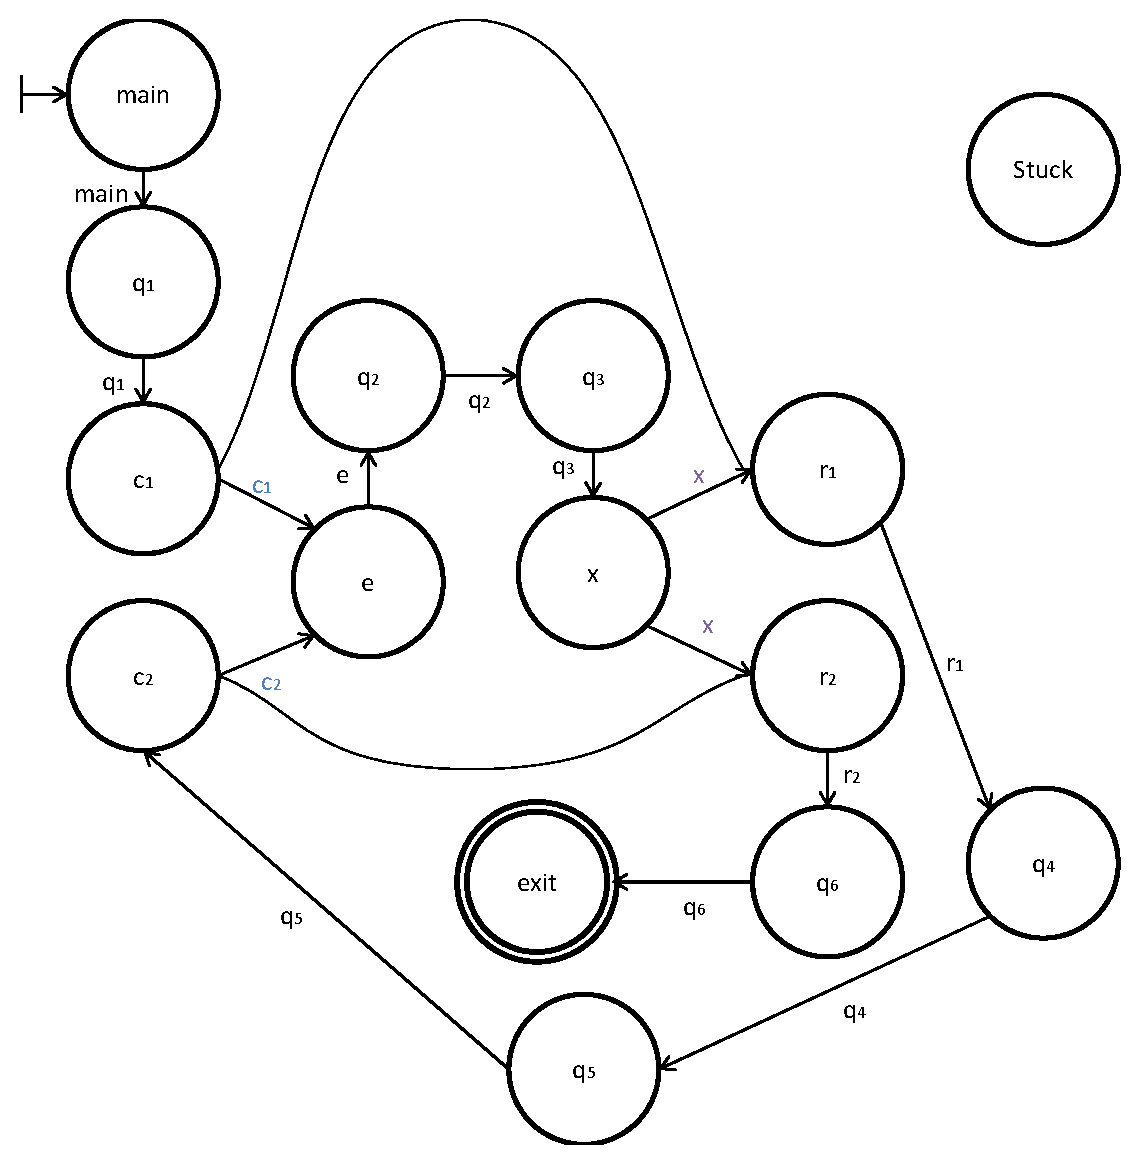
\includegraphics[width=12cm]{Figures/Figure23}
  \caption{An example NWA.}
  \label{Fig:NWAtoPDS1}
\end{figure}

\subsubsection{1. Forwards Flow Stacking Calls}

\noindent The conversion is performed by:



\begin{mathpar}

{\inferrule*%%[left=\textsc{States}]
  { }
  {p \in P}
}
\and 
{\inferrule*
  { (q_x,q_c,\sigma,q_r) \in \delta_r }
  { p_{q_x} \in P }
}
\and
{\inferrule*
  { q \in Q }
  { q \in \Gamma }
}
\and 
{\inferrule*%%[left=\textsc{Internal}]
  { (q,\sigma,q') \in \delta_i }
  { \langle p,q \rangle \stackrel{w_1}{\hookrightarrow} \langle p,q' \rangle \in \Delta_1 }
}
\and
{\inferrule*%%[left=\textsc{Call}]
  { (q_c,\sigma, q_e) \in \delta_c }
  {  \langle p,q_c \rangle \stackrel{w_2}{\hookrightarrow} \langle p, q_e \hspace{.1cm} q_c \rangle\in \Delta_2 }
}
\and
{\inferrule*%%[left=\textsc{Return}]
  { (q_x,q_c,\sigma,q_r) \in \delta_r }
  { \langle p,q_x \rangle \stackrel{w_0}{\hookrightarrow} \langle p_{q_x},\epsilon \rangle \in \Delta_0 \\
   \langle p_{q_x},q_c \rangle \stackrel{w_3}{\hookrightarrow} \langle p,q_r \rangle\in \Delta_1  }
}
\end{mathpar}
\begin{align*}
\text{where }
w_0 & = \begin{cases}
        \mathtt{wg.getOne}(), & \text{if } \sigma = \epsilon \\
        \mathtt{wg.getWildWeight}(q,CI_q,q',CI_{q'}), & \text{if } \sigma = \text{*} \\
        \mathtt{wg.getWeight}(q_x,CI_{q_x},\sigma,\mathtt{EXIT\_TO\_RET},q_r,CI_{q_r}), & \text{otherwise}
      \end{cases}  \\
w_1 &= \begin{cases}
         \mathtt{wg.getOne}(), & \text{if } \sigma = \epsilon \\
         \mathtt{wg.getWildWeight}(q,CI_q,q',CI_{q'}), & \text{if } \sigma = \text{*} \\
         \mathtt{wg.getWeight}(q,CI_q,\sigma,\mathtt{INTRA},q',CI_{q'}), & \text{otherwise}
      \end{cases} \\
w_2 &= \begin{cases}
         \mathtt{wg.getOne}(), & \text{if } \sigma = \epsilon \\
         \mathtt{wg.getWildWeight}(q,CI_q,q',CI_{q'}), & \text{if } \sigma = \text{*} \\
         \mathtt{wg.getWeight}(q_c,CI_{q_c},\sigma,\mathtt{CALL\_TO\_ENTRY},q_e,CI_{q_e}), & \text{otherwise}
      \end{cases} \\
w_3 &= \mathtt{wg.getOne}() 
\end{align*}


\noindent Consider, as an example, converting the NWA in Figure
\ref{Fig:NWAtoPDS5} into a WPDS. The WPDS resulting from converting the NWA
shown in Figure \ref{Fig:NWAtoPDS1} into a WPDS is shown in Figure
\ref{Fig:NWAtoPDS4}. \\

\begin{figure}[htbp]
  \centering
    \begin{itemize}
      \centering
      \item{ $\langle p,main \rangle \hookrightarrow \langle p,q_1 \rangle$}
      \item{ $\langle p,q_1 \rangle \hookrightarrow \langle p,c_1 \rangle$}
      \item{ $\langle p,e \rangle \hookrightarrow \langle p,q_2 \rangle$}
      \item{ $\langle p,q_2 \rangle \hookrightarrow \langle p,q_3 \rangle$}
      \item{ $\langle p,q_3 \rangle \hookrightarrow \langle p,x \rangle$}
      \item{ $\langle p,r_1 \rangle \hookrightarrow \langle p,q_4 \rangle$}
      \item{ $\langle p,q_4 \rangle \hookrightarrow \langle p,q_5 \rangle$}
      \item{ $\langle p,q_5 \rangle \hookrightarrow \langle p,c_2 \rangle$}
      \item{ $\langle p,r_2 \rangle \hookrightarrow \langle p,q_6 \rangle$}
      \item{ $\langle p,q_6 \rangle \hookrightarrow \langle p,exit \rangle$}
      \item{ $\langle p,c_1 \rangle \hookrightarrow \langle p,e \hspace{.1cm} c_1 \rangle$}
      \item{ $\langle p,c_2 \rangle \hookrightarrow \langle p,e \hspace{.1cm} c_2 \rangle$}
      \item{ $\langle p,x \rangle \hookrightarrow \langle p_x, \epsilon \rangle$}
      \item{ $\langle p_x,c_1 \rangle \hookrightarrow \langle p,r_1 \rangle$}
      \item{ $\langle p,x \rangle \hookrightarrow \langle p_x, \epsilon \rangle$}
      \item{ $\langle p_x,c_2 \rangle \hookrightarrow \langle p,r_2 \rangle$}
    \end{itemize}
  \caption{The WPDS resulting from converting the NWA shown in Figure \ref{Fig:NWAtoPDS1} into a WPDS.}
  \label{Fig:NWAtoPDS4}
\end{figure}

\subsubsection{2. Backwards Flow Stacking Calls}

\noindent The conversion is performed by:



\begin{mathpar}
{\inferrule*%%[left=\textsc{States}]
  { }
  {p \in P}
}
\and 
{\inferrule*
  { (q_c,\sigma,q_e) \in \delta_c }
  { p_{q_e} \in P }
}
\and
{\inferrule*
  { q \in Q }
  { q \in \Gamma }
}
\and 
{\inferrule*%%[left=\textsc{Internal}]
  { (q,\sigma,q') \in \delta_i }
  { \langle p,q' \rangle \stackrel{w_1}{\hookrightarrow} \langle p,q \rangle \in \Delta_1 }
}
\and  
{\inferrule*%%[left=\textsc{Call}]
  { (q_c,\sigma, q_e) \in \delta_c \\ (q_x,q_c,\gamma,q_r) \in \delta_r }
  { \langle p,q_e \rangle \stackrel{w_0}{\hookrightarrow} \langle p_{q_e},\epsilon \rangle \in \Delta_0 \\
    \langle p_{q_e},q_r \rangle \stackrel{w_3}{\hookrightarrow} \langle p,q_c  \rangle \in \Delta_1 }
}
\and
{\inferrule*%%[left=\textsc{Return}]
  { (q_x,q_c,\sigma,q_r) \in \delta_r }
  {  \langle p,q_r \rangle \stackrel{w_2}{\hookrightarrow} \langle p,q_x \hspace{.1cm} q_r
  \rangle \in \Delta_2 }
}
\end{mathpar}
\begin{align*}
\text{where }
w_0 &= \begin{cases}
           \mathtt{wg.getOne}(), & \text{if } \sigma = \epsilon \\
           \mathtt{wg.getWildWeight}(q_c,CI_{q_c},q_e,CI_{q_e}), & \text{if } \sigma = \text{*} \\
           \mathtt{wg.getWeight}(q_c,CI_{q_c},\sigma, \mathtt{CALL\_TO\_ENTRY},q_e,CI_{q_e}), & \text{otherwise}
      \end{cases} \\
w_1 &= \begin{cases}
           \mathtt{wg.getOne}(), & \text{if } \sigma = \epsilon \\
           \mathtt{wg.getWildWeight}(q,CI_q,q',CI_{q'}), & \text{if } \sigma = \text{*} \\
           \mathtt{wg.getWeight}(q,CI_q,\sigma, \mathtt{INTRA},q',CI_{q'}), & \text{otherwise}
       \end{cases} \\
w_2 &= \begin{cases}
          \mathtt{wg.getOne}(), & \text{if } \sigma = \epsilon \\
          \mathtt{wg.getWildWeight}(q_x,CI_{q_x},q_r,CI_{q_r}), & \text{if } \sigma = \text{*} \\
          \mathtt{wg.getWeight}(q_x,CI_{q_x},\sigma, \mathtt{EXIT\_TO\_RET},q_r,CI_{q_r}), & \text{otherwise}
      \end{cases} \\
w_3 &= \mathtt{wg.getOne}()
\end{align*}




\noindent Consider, as an example, converting the NWA in Figure
\ref{Fig:NWAtoPDS1} into a backwards flow WPDS.  The WPDS resulting from
converting the NWA shown in Figure \ref{Fig:NWAtoPDS1} into a backwards flow
WPDS is shown in Figure \ref{Fig:NWAtoPDS5}.  Note:
\texttt{NWAtoBackwardsPDScalls(A)} = \texttt{NWAtoPDScalls(reverse(A))}.  \\

\begin{figure}[htbp]
  \centering
    \begin{itemize}
      \centering
      \item{ $\langle p,q_1 \rangle \hookrightarrow \langle p,main \rangle$}
      \item{ $\langle p,c_1 \rangle \hookrightarrow \langle p,q_1 \rangle$}
      \item{ $\langle p,q_2 \rangle \hookrightarrow \langle p,e \rangle$}
      \item{ $\langle p,q_3 \rangle \hookrightarrow \langle p,q_2 \rangle$}
      \item{ $\langle p,x \rangle \hookrightarrow \langle p,q_3 \rangle$}
      \item{ $\langle p,q_4 \rangle \hookrightarrow \langle p,r_1 \rangle$}
      \item{ $\langle p,q_5 \rangle \hookrightarrow \langle p,q_4 \rangle$}
      \item{ $\langle p,c_2 \rangle \hookrightarrow \langle p,q_5 \rangle$}
      \item{ $\langle p,q_6 \rangle \hookrightarrow \langle p,r_2 \rangle$}
      \item{ $\langle p,exit \rangle \hookrightarrow \langle p,q_6 \rangle$}
      \item{ $\langle p,r_1 \rangle \hookrightarrow \langle p,x \hspace{.1cm} r_1 \rangle$}
      \item{ $\langle p,r_2 \rangle \hookrightarrow \langle p,x \hspace{.1cm} r_2 \rangle$}
      \item{ $\langle p,e \rangle \hookrightarrow \langle p_e, \epsilon \rangle$}
      \item{ $\langle p_e,r_1 \rangle \hookrightarrow \langle p,c_1 \rangle$}
      \item{ $\langle p,e \rangle \hookrightarrow \langle p_e, \epsilon \rangle$}
      \item{ $\langle p_e,r_2 \rangle \hookrightarrow \langle p,c_2 \rangle$}
    \end{itemize}
  \caption{The WPDS resulting from converting the NWA shown in Figure \ref{Fig:NWAtoPDS1} into a WPDS.}
  \label{Fig:NWAtoPDS5}
\end{figure}

\subsubsection{3. Forwards Flow Stacking Returns}

\noindent The conversion is performed by:


\begin{mathpar}
{\inferrule*%%[left=\textsc{States}]
  { }
  {p \in P}
}
\and 
{\inferrule*
  { (q_x,q_c,\sigma,q_r) \in \delta_r }
  { p_{q_x} \in P }
}
\and
{\inferrule*
  { q \in Q }
  { q \in \Gamma }
}
\and 
{\inferrule*%%[left=\textsc{Internal}]
  { (q,\sigma,q') \in \delta_i }
  { \langle p,q  \rangle \stackrel{w_1}{\hookrightarrow} \langle p,q' \rangle \in \Delta_1 }
}
\and
{\inferrule*%%[left=\textsc{Call}]
  { (q_c,\sigma, q_e) \in \delta_c \\ (q_x,q_c,\gamma,q_r) \in \delta_r }
  { \langle p,q_c \rangle \stackrel{w_2}{\hookrightarrow}  \langle p, q_e \hspace{.1cm} q_r \rangle \in \Delta_2 }
}
\and 
{\inferrule*%%[left=\textsc{Return}]
  { (q_x,q_c,\sigma,q_r) \in \delta_r }
  { \langle p,q_x \rangle \stackrel{w_0}{\hookrightarrow} \langle p_{q_x},\epsilon \rangle \in  \Delta_0 \\
    \langle  p_{q_x},q_r \rangle \stackrel{w_3}{\hookrightarrow} \langle p,q_r \rangle \in \Delta_1 }
}
\end{mathpar}
\begin{align*}
\text{where }
w_0 &= \mathtt{wg.getOne}() \\
w_1 &= \begin{cases}
           \mathtt{wg.getOne}(), & \text{if } \sigma = \epsilon \\
           \mathtt{wg.getWildWeight}(q,CI_q,q',CI_{q'}), & \text{if } \sigma = \text{*} \\
           \mathtt{wg.getWeight}(q,CI_q,\sigma, \mathtt{INTRA},q',CI_{q'}), & \text{otherwise}
       \end{cases} \\
w_2 &= \begin{cases}
           \mathtt{wg.getOne}(), & \text{if } \sigma = \epsilon \\
           \mathtt{wg.getWildWeight}(q_c,CI_{q_c},q_e,CI_{q_e}), & \text{if } \sigma = \text{*} \\
           \mathtt{wg.getWeight}(q_c,CI_{q_c},\sigma, \mathtt{CALL\_TO\_ENTRY},q_e,CI_{q_e}), & \text{otherwise}
      \end{cases} \\
w_3 &= \begin{cases}
          \mathtt{wg.getOne}(), & \text{if } \sigma = \epsilon \\
          \mathtt{wg.getWildWeight}(q_x,CI_{q_x},q_r,CI_{q_r}), & \text{if } \sigma = \text{*} \\
          \mathtt{wg.getWeight}(q_x,CI_{q_x},\sigma, \mathtt{EXIT\_TO\_RET},q_r,CI_{q_r}), & \text{otherwise}
      \end{cases} 
\end{align*}


\noindent Consider, as an example, converting the NWA in Figure
\ref{Fig:NWAtoPDS1} into a WPDS.  The WPDS resulting from converting the WPDS
shown in Figure \ref{Fig:NWAtoPDS1} into a WPDS is shown in Figure
\ref{Fig:NWAtoPDS2}. \\

\begin{figure}[htbp]
  \centering
    \begin{itemize}
      \centering
      \item{ $\langle p,main \rangle \hookrightarrow \langle p,q_1 \rangle$}
      \item{ $\langle p,q_1 \rangle \hookrightarrow \langle p,c_1 \rangle$}
      \item{ $\langle p,e \rangle \hookrightarrow \langle p,q_2 \rangle$}
      \item{ $\langle p,q_2 \rangle \hookrightarrow \langle p,q_3 \rangle$}
      \item{ $\langle p,q_3 \rangle \hookrightarrow \langle p,x \rangle$}
      \item{ $\langle p,r_1 \rangle \hookrightarrow \langle p,q_4 \rangle$}
      \item{ $\langle p,q_4 \rangle \hookrightarrow \langle p,q_5 \rangle$}
      \item{ $\langle p,q_5 \rangle \hookrightarrow \langle p,c_2 \rangle$}
      \item{ $\langle p,r_2 \rangle \hookrightarrow \langle p,q_6 \rangle$}
      \item{ $\langle p,q_6 \rangle \hookrightarrow \langle p,exit \rangle$}
      \item{ $\langle p,c_1 \rangle \hookrightarrow \langle p,e \hspace{.1cm} r_1 \rangle$}
      \item{ $\langle p,c_2 \rangle \hookrightarrow \langle p,e \hspace{.1cm} r_2 \rangle$}
      \item{ $\langle p,x \rangle \hookrightarrow \langle p_x, \epsilon \rangle$}
      \item{ $\langle p_x,r_1 \rangle \hookrightarrow \langle p,r_1 \rangle$}
      \item{ $\langle p,x \rangle \hookrightarrow \langle p_x, \epsilon \rangle$}
      \item{ $\langle p_x,r_2 \rangle \hookrightarrow \langle p,r_2 \rangle$}
    \end{itemize}
  \caption{The WPDS resulting from converting the NWA shown in Figure \ref{Fig:NWAtoPDS1} into a WPDS.}
  \label{Fig:NWAtoPDS2}
\end{figure}

\subsubsection{4. Backwards Flow Stacking Returns}

\noindent The conversion is performed by:



\begin{mathpar}
{\inferrule*[left=\textsc{States}]
  { }
  {p \in P}
}
\and 
{\inferrule*
  { (q_c,\sigma,q_e) \in \delta_c }
  { p_{q_e} \in P }
}
\and
{\inferrule*
  { q \in Q }
  { q \in \Gamma }
}
\and 
{\inferrule*%%[left=\textsc{Internal}]
  { (q,\sigma,q') \in \delta_i }
  { \langle  p,q' \rangle \stackrel{w_1}{\hookrightarrow} \langle p,q \rangle \in \Delta_1 }
}
\and
{\inferrule*%%[left=\textsc{Call}]
  { (q_c,\sigma, q_e) \in \delta_c }
  { \langle  p,q_e \rangle \stackrel{w_0}{\hookrightarrow} \langle p_{q_e},\epsilon \rangle \in \Delta_0 \\
    \langle  p_{q_e},q_c \rangle \stackrel{w_3}{\hookrightarrow} \langle p,q_c \rangle \in \Delta_1  }
}
\and 
{\inferrule*%%[left=\textsc{Return}]
  { (q_x,q_c,\sigma,q_r) \in \delta_r }
  { \langle p,q_r \rangle \stackrel{w_2}{\hookrightarrow} \langle p,q_x \hspace{.1cm} q_c  \rangle \in \Delta_2 }
}
\end{mathpar}
\begin{align*}
\text{where }
w_0 &= \mathtt{wg.getOne}() \\
w_1 &= \begin{cases}
           \mathtt{wg.getOne}(), & \text{if } \sigma = \epsilon \\
           \mathtt{wg.getWildWeight}(q,CI_q,q',CI_{q'}), & \text{if } \sigma = \text{*} \\
           \mathtt{wg.getWeight}(q,CI_q,\sigma, \mathtt{INTRA},q',CI_{q'}), & \text{otherwise}
       \end{cases} \\
w_2 &= \begin{cases}
          \mathtt{wg.getOne}(), & \text{if } \sigma = \epsilon \\
          \mathtt{wg.getWildWeight}(q_x,CI_{q_x},q_r,CI_{q_r}), & \text{if } \sigma = \text{*} \\
          \mathtt{wg.getWeight}(q_x,CI_{q_x},\sigma, \mathtt{EXIT\_TO\_RET},q_r,CI_{q_r}), & \text{otherwise}
      \end{cases} \\
w_3 &= \begin{cases}
           \mathtt{wg.getOne}(), & \text{if } \sigma = \epsilon \\
           \mathtt{wg.getWildWeight}(q_c,CI_{q_c},q_e,CI_{q_e}), & \text{if } \sigma = \text{*} \\
           \mathtt{wg.getWeight}(q_c,CI_{q_c},\sigma, \mathtt{CALL\_TO\_ENTRY},q_e,CI_{q_e}), & \text{otherwise}
      \end{cases} 
\end{align*}



\begin{enumerate}

\item For each $(q,\sigma,q')$ $\in \delta_i$ in the NWA, adding $\langle
  p,q' \rangle \hookrightarrow \langle p,q \rangle$ to $\Delta_1$ of the WPDS
  (with weight
  \texttt{wg.getWeight($q$,$CI_q$,$\sigma$,INTRA,$q'$,$CI_{q'}$}) or
  \texttt{wg.getWildWeight($q$,$CI_q$,$q'$,$CI_{q'}$)}, depending on $\sigma$
  ).

\item For each $(q_c,\sigma, q_e)$ $\in \delta_c$ in the NWA, adding $\langle
  p,q_e \rangle \hookrightarrow \langle p_{q_e},\epsilon \rangle$ to
  $\Delta_0$ of the WPDS (with weight \texttt{wg.getOne()} ) and $\langle
  p_{q_e},q_c \rangle \hookrightarrow \langle p,q_c \rangle$ to $\Delta_1$ of
  the WPDS (with weight
  \texttt{wg.getWeight($q_c$,$CI_{q_c}$,$\sigma$,CALL\_TO\_ENTRY,$q_e$,$CI_{q_e}$)}
  or \texttt{wg.getWildWeight($q_c$,$CI_{q_c}$,$q_e$,$CI_{q_e}$)}, depending
  on $\sigma$).

\item For each $(q_x,q_c,\sigma,q_r)$ $\in \delta_r$ in the NWA, adding
  $\langle p,q_r \rangle \hookrightarrow \langle p,q_x \hspace{.1cm} q_c
  \rangle$ to $\Delta_2$ of the WPDS (with weight
  \texttt{wg.getWeight($q_x$,$CI_{q_x}$,$\sigma$,EXIT\_TO\_RET,$q_r$,$CI_{q_r}$)}
  or \texttt{wg.getWildWeight($q_x$,$CI_{q_x}$,$q_r$,$CI_{q_r}$)}, depending
  on $\sigma$).
\end{enumerate}

\noindent Consider, as an example, converting the NWA in Figure
\ref{Fig:NWAtoPDS3} into a backwards flow WPDS.  The WPDS resulting from
converting the WPDS shown in Figure \ref{Fig:NWAtoPDS1} into a backwards flow
WPDS is shown in Figure \ref{Fig:NWAtoPDS3}. \\

\begin{figure}[htbp]
  \centering
    \begin{itemize}
      \centering
      \item{ $\langle p,q_1 \rangle \hookrightarrow \langle p,main \rangle$}
      \item{ $\langle p,c_1 \rangle \hookrightarrow \langle p,q_1 \rangle$}
      \item{ $\langle p,q_2 \rangle \hookrightarrow \langle p,e \rangle$}
      \item{ $\langle p,q_3 \rangle \hookrightarrow \langle p,q_2 \rangle$}
      \item{ $\langle p,x \rangle \hookrightarrow \langle p,q_3 \rangle$}
      \item{ $\langle p,q_4 \rangle \hookrightarrow \langle p,r_1 \rangle$}
      \item{ $\langle p,q_5 \rangle \hookrightarrow \langle p,q_4 \rangle$}
      \item{ $\langle p,c_2 \rangle \hookrightarrow \langle p,q_5 \rangle$}
      \item{ $\langle p,q_6 \rangle \hookrightarrow \langle p,r_2 \rangle$}
      \item{ $\langle p,exit \rangle \hookrightarrow \langle p,q_6 \rangle$}
      \item{ $\langle p,r_1 \rangle \hookrightarrow \langle p,x \hspace{.1cm} c_1 \rangle$}
      \item{ $\langle p,r_2 \rangle \hookrightarrow \langle p,x \hspace{.1cm} c_2 \rangle$}
      \item{ $\langle p,e \rangle \hookrightarrow \langle p_e, \epsilon \rangle$}
      \item{ $\langle p_e,c_1 \rangle \hookrightarrow \langle p,c_1 \rangle$}
      \item{ $\langle p,e \rangle \hookrightarrow \langle p_e, \epsilon \rangle$}
      \item{ $\langle p_e,c_2 \rangle \hookrightarrow \langle p,c_2 \rangle$}
    \end{itemize}
  \caption{The WPDS resulting from converting the NWA shown in Figure
    \ref{Fig:NWAtoPDS1} into a WPDS.}
  \label{Fig:NWAtoPDS3}
\end{figure}


